\documentclass[xelatex,12pt]{beamer}
\usepackage{pgfpages}
\usepackage{fontspec}
\usepackage{xunicode}
\usepackage{polyglossia}
\PolyglossiaSetup{french}{indentfirst=false}
\usepackage[french=guillemets]{csquotes}
\usepackage{xpatch}
\usepackage{diagbox}

\setmainlanguage{french}
\xapptocmd\ttfamily{\XeTeXinterchartokenstate=0 }{}{}
\newcommand{\nospace}[1]{\texttt{#1}}

\usepackage{algorithm}
\usepackage[noend]{algpseudocode}
    \newcounter{lastenum}
    \newcommand{\mtpause}{\setcounter{lastenum}{\value{enumi}}}
    \newcommand{\mtresume}{\setcounter{enumi}{\value{lastenum}}}
\resetcounteronoverlays{lastenum}

\usepackage[backend=biber, style=chem-acs]{biblatex}
\addbibresource{Modele.bib} 
\setbeamertemplate{bibliography item}[triangle]


 
\usepackage{multirow}% row fusion
\usepackage{array} % column fusion
\usepackage{xfrac} % small fractions
\usepackage{adjustbox}
\usepackage{listings}

\usepackage{color}
\definecolor{gray}{rgb}{0.4,0.4,0.4}
\definecolor{darkblue}{rgb}{0.0,0.0,0.6}
\definecolor{cyan}{rgb}{0.0,0.6,0.6}

\usetheme{Warsaw}

\setbeamertemplate{frametitle}{\nointerlineskip  
    \begin{beamercolorbox}[wd=\paperwidth,ht=2.75ex,dp=1.375ex]{frametitle}
        \hspace*{2ex}\insertframetitle \hfill {\small\insertframenumber/\inserttotalframenumber} \hspace*{1ex}%
    \end{beamercolorbox}}

\usecolortheme{wolverine}

\setbeameroption{hide notes} % Only slides
%\setbeameroption{show only notes} % Only notes
%\setbeameroption{show notes on second screen=right} % Both

 \titlegraphic{\vspace{-1cm}
      
\includegraphics[width=2.5cm]{images/logo_paris_8.png}\hspace*{4.75cm}~%
      \hfill
      
\includegraphics[width=2.5cm]{images/tc_logo.jpeg}
}

 
\title{Classification et affectation des transactions aux magasins des détaillants}
\subtitle{stage effectué chez Transaction Connect}
\author[\textsc{Komlan DANTODJI}]{\textsc{Komlan Jean-Marie DANTODJI}}
\institute{\normalsize Université Paris 8, LIASD\\
Encadrante : Mme Rakia JAZIRI\\
Tuteur : Mr Thomas MOULIN
}
 
\beamertemplatenavigationsymbolsempty
\setbeamertemplate{blocks}[rounded][shadow=true]
\setbeamerfont{page number in head/foot}{size=\large}

\begin{document}
{ \setbeamertemplate{headline}{}
  \setbeamertemplate{footline}{}
  \begin{frame}
  \titlepage
  \end{frame}

\note{
}
}

\begin{frame}{Plan}
  \tableofcontents[sectionstyle=show/show, hidesubsections]
\note{
}  
\end{frame}

\section{Introduction}
\subsection{Présentation de l'entreprise}
\begin{frame}{Transaction Connect}
\begin{itemize}
		\item Start Up de B2B2C
		\item Editeur de solution numérique basé sur la donnée de paiement
		\item Solution déployée dans 10 pays européens et compte 60 clients
\end{itemize}
\end{frame}

\subsection{Solutions proposées}
\begin{frame}{Solutions proposées}
\begin{itemize}
		\item Transaction Connect signe des contrats avec des foncières
		\item Transformation de tout moyen de paiement en carte de fidélité
		\item Amélioration de la connaissance client aux acteurs du commerce physique
		\item Notification et Validation des récompenses aux clients acheteurs
\end{itemize}
\end{frame}

\begin{frame}{Les modes d'intégrations des Clients Business}
\begin{figure}[H]
    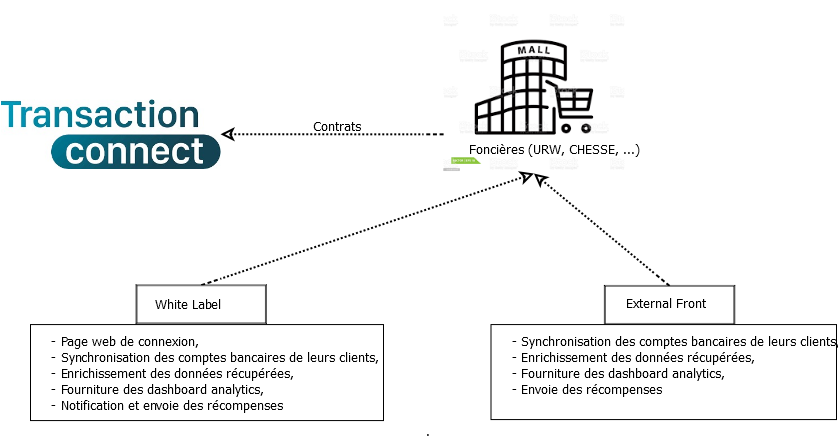
\includegraphics[width=11cm,height=4.8cm]{images/business_links.png}
    \caption{ modes d'intégration B}
    \label{fig:L1}
\end{figure}
\end{frame}
\begin{frame}{Les modes de connexion des Clients}
\begin{figure}[H]
    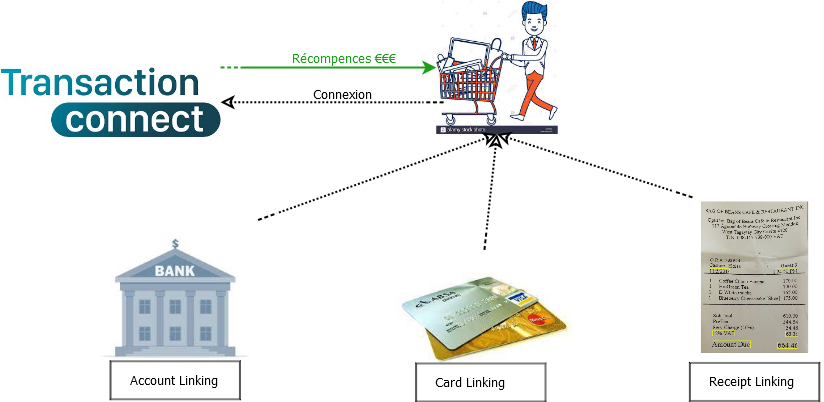
\includegraphics[width=11cm,height=4.8cm]{images/client_links.png}
    \caption{ Mode de connexion des trannsactions}
    \label{fig:L1}
\end{figure}
\end{frame}

\section{Contexte} % pour l'exposé final, commenter
%\subsection{Contexte} % pour l'exposé final, décommenter

\begin{frame}{Contexte RH}
  \begin{itemize}
  \item nom du service
  \item composition du service
  \item tâches
  \end{itemize}
\end{frame}

\begin{frame}{Contexte technique}
  \begin{itemize}
  \item contexte matériel
  \item contexte logiciel
  \item contraintes
  \end{itemize}
\end{frame}

\section{Problématique}

\subsection{Objectif}

\begin{frame}{Problème}
  \begin{itemize}
  \item Classification des transactions des clients
  \item Affectation de transactions à un magasin
  \end{itemize}
\end{frame}

\subsection{Données}
\begin{frame}{Features Engineering }
\begin{figure}[H]
    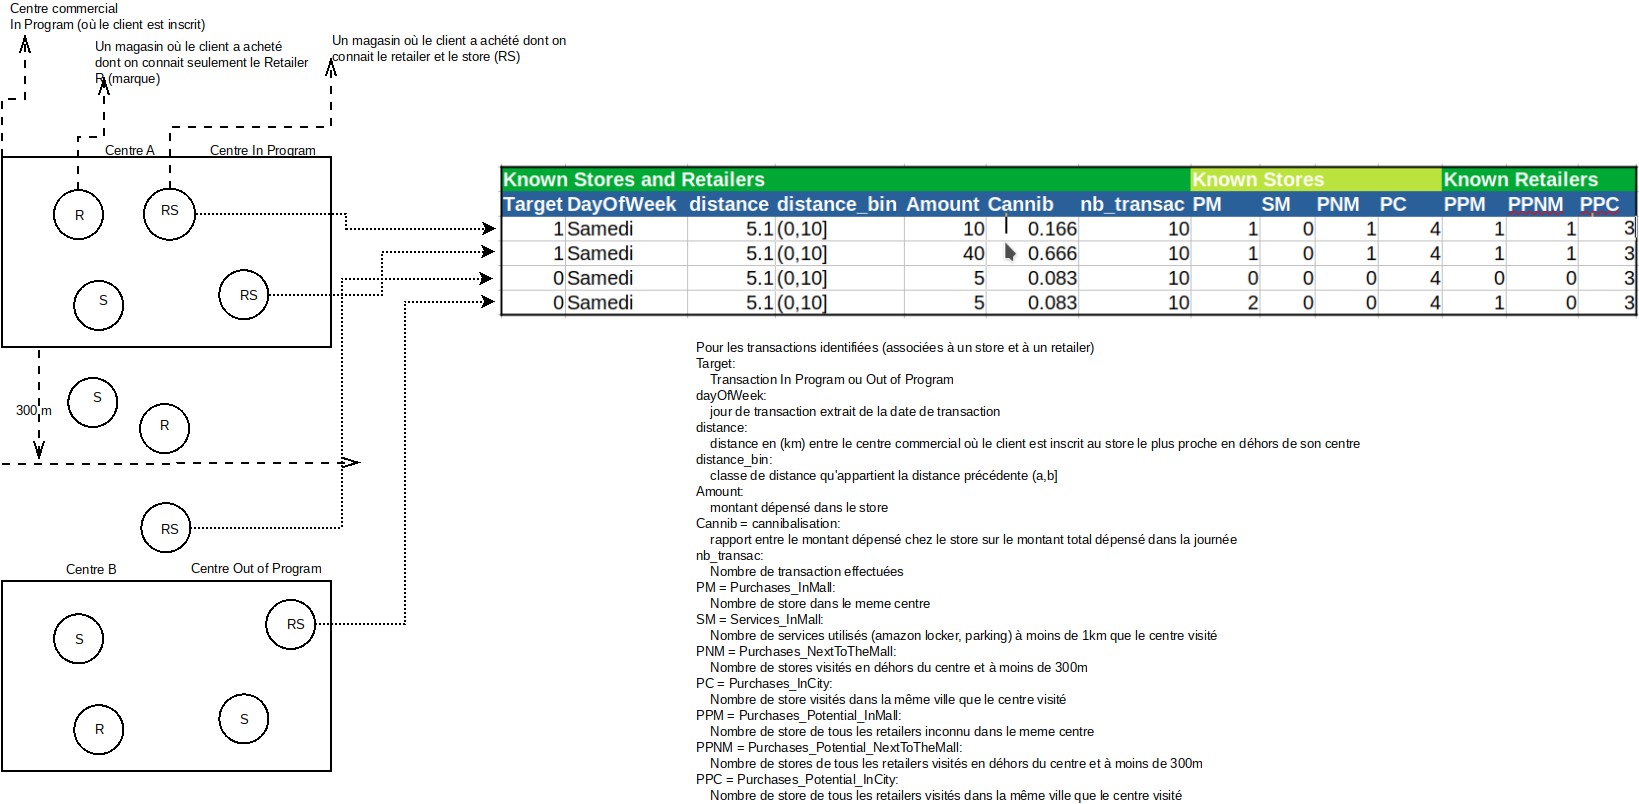
\includegraphics[width=11.5cm,height=5.5cm]{images/feature_engineering.png}
    \label{fig:L1}
\end{figure}
\end{frame}

\begin{frame}{Jeu de données}
\begin{figure}[H]
    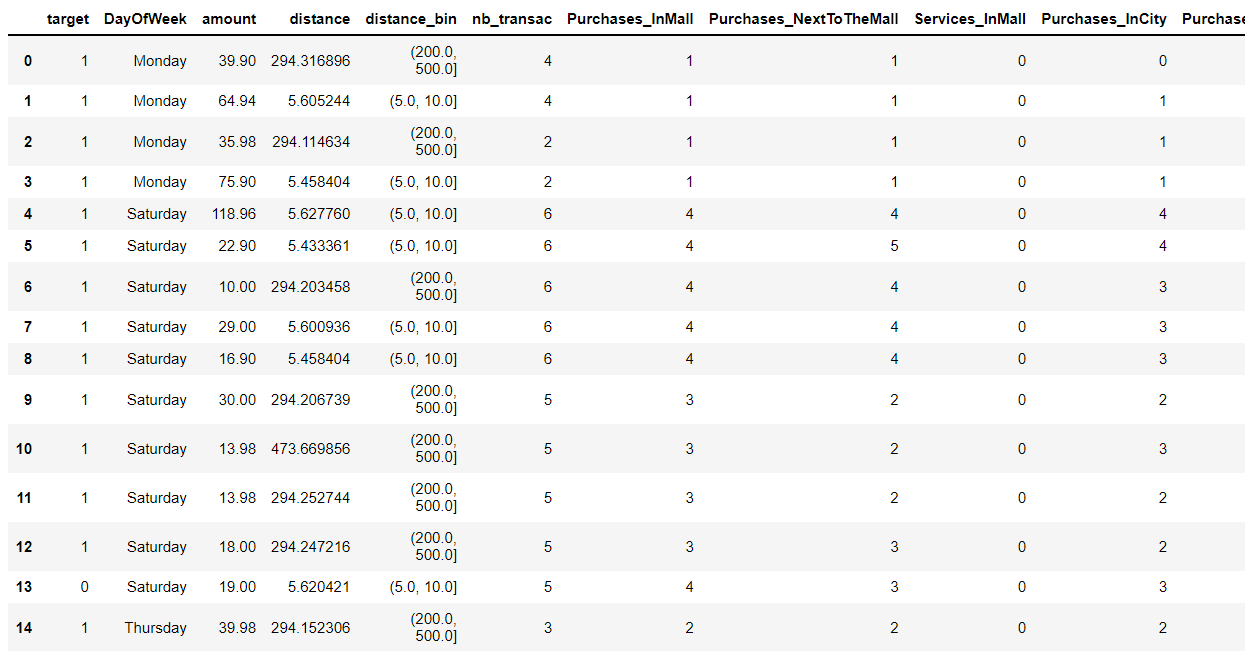
\includegraphics[width=12cm,height=4.8cm]{images/dataset_1.png}
    \caption{ Transactions considérées}
    \label{fig:L1}
\end{figure}
\end{frame}
\begin{frame}{Jeu de données}
\begin{figure}[H]
    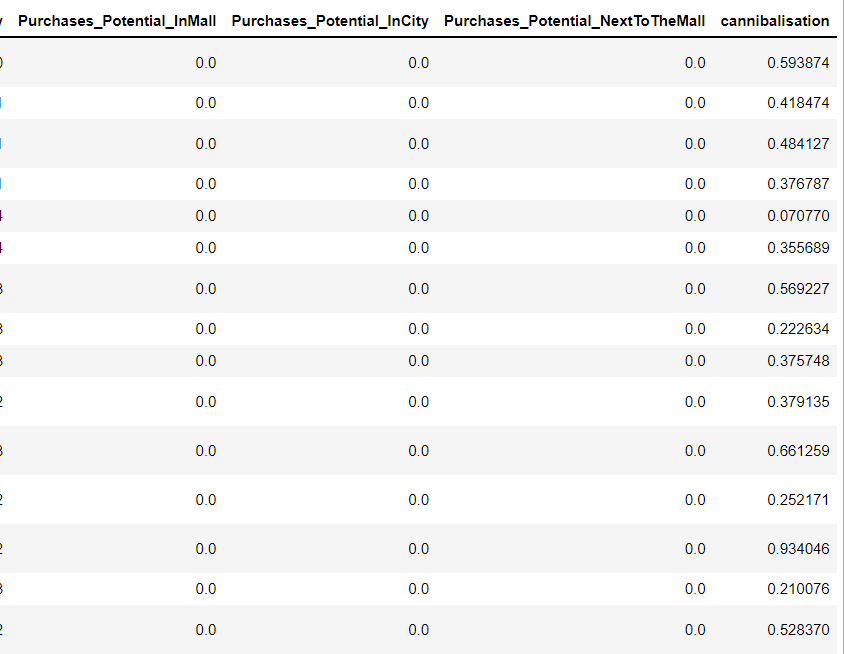
\includegraphics[width=11cm,height=4.8cm]{images/dataset_2.png}
    \caption{ Transactions considérées}
    \label{fig:L1}
\end{figure}
\end{frame} 

\begin{frame}{Données}
  \begin{itemize}
  \item 483.725 lignes, 14 colonnes
  \item Données claculées grace au scoring des transactions 
  \end{itemize}
\end{frame}

\section{État de l'art}
\subsection{Catégories d'algorithmes utilisés}
\begin{frame}{Catégories d'algorithmes utilisés}
  \begin{itemize}
  \item Support Vector Machine
  \item Decision Tree
  \item Random Forest
  \item K Nearest Neighbor
  \item Gradient boosting (XGBoost)
  \item Regression Logistique
  \item Naive Bayes
  \end{itemize}
\end{frame}
\subsection{Support Vector Machine}
\begin{frame}{Support Vector Machine}
	\begin{figure}[H]
    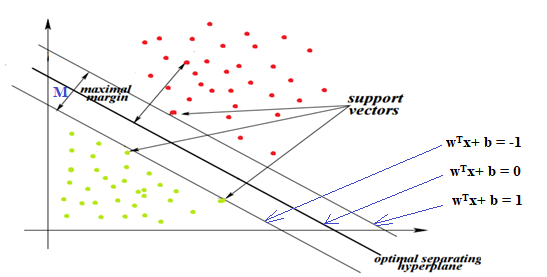
\includegraphics[width=\linewidth, height=4.8cm]{images/svm_separate.png}
    \caption{Détermination de l’hyperplan}
    \label{fig:L1}
\end{figure}
\end{frame}

\subsection{SVM: Déterminsation d'hyperplan}
\begin{frame}{SVM: Déterminsation d'hyperplan}
 $x_0$ et $x_1$ deux vecteurs supports aux deux extrémités,\\
Soit l' hyperplant $$(P): w^Tx+b=0$$

$$M = d(x_{0},P)+d(x_{1},P) = \frac{\mid{w^{T}x_{0}+b}\mid}{\sqrt{w^{T}w} } + \frac{\mid{w^{T}x_{1}+b}\mid}{\sqrt{w^{T}w} } $$

$$ = \frac{\mid{1}\mid}{\sqrt{w^{T}w} } + \frac{\mid{-1}\mid}{\sqrt{w^{T}w}} = \frac{2}{\sqrt{w^{T}w} }$$  
\par Maximiser M revient à minimiser $$\frac{\sqrt{w^{T}w}}{2} = \frac{\|w\|}{2}$$
\end{frame}
\subsection{Arbre de décision}
\begin{frame}{Arbre de décision}
	\begin{figure}[H]
    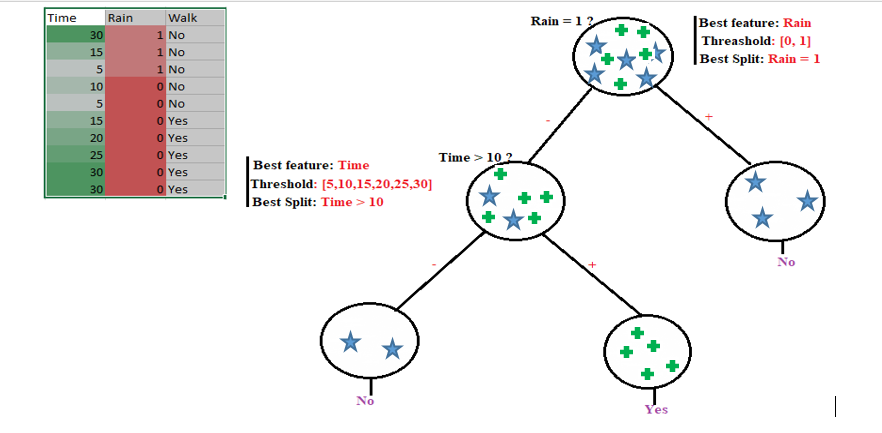
\includegraphics[width=\linewidth, height=4.8cm]{images/decision_tree_formular.png}
    \caption{Arbre de décision}
    \label{fig:L1}
\end{figure}
\end{frame}
\begin{frame}{Arbre de décision}
 $$ Soit \, X_i \,(label) \in ["Yes","No"] $$
$$ Posons\, P(X_i) = \frac{nb\_label\_i\_in\_node}{total\_population}$$
$$ Pour\,Entropie:\, E = - \sum_{i=0}^{nb\_labels} P(X_i) * log_2(P(X_i))$$ 
$$ Pour\,Gini:\, G = 1 - \sum_{i=0}^{nb\_labels} P(X_i)^2$$ 
\end{frame}
\begin{frame}{Arbre de décision} 
Déterminer la meilleure variable et coupure qui correspond au Max(IG):
$$IG = E(parent) - \sum_{i=0}^{nb\_childs} \frac{total\_population\_in\_node}{total\_population}E(child\_i)$$
$$IG = G(parent) - \sum_{i=0}^{nb\_childs} \frac{total\_population\_in\_node}{total\_population}G(child\_i)$$
\end{frame}

\subsection{Forêst aléatoire}
\begin{frame}{Forêt aléatoire}
	\begin{figure}[H]
    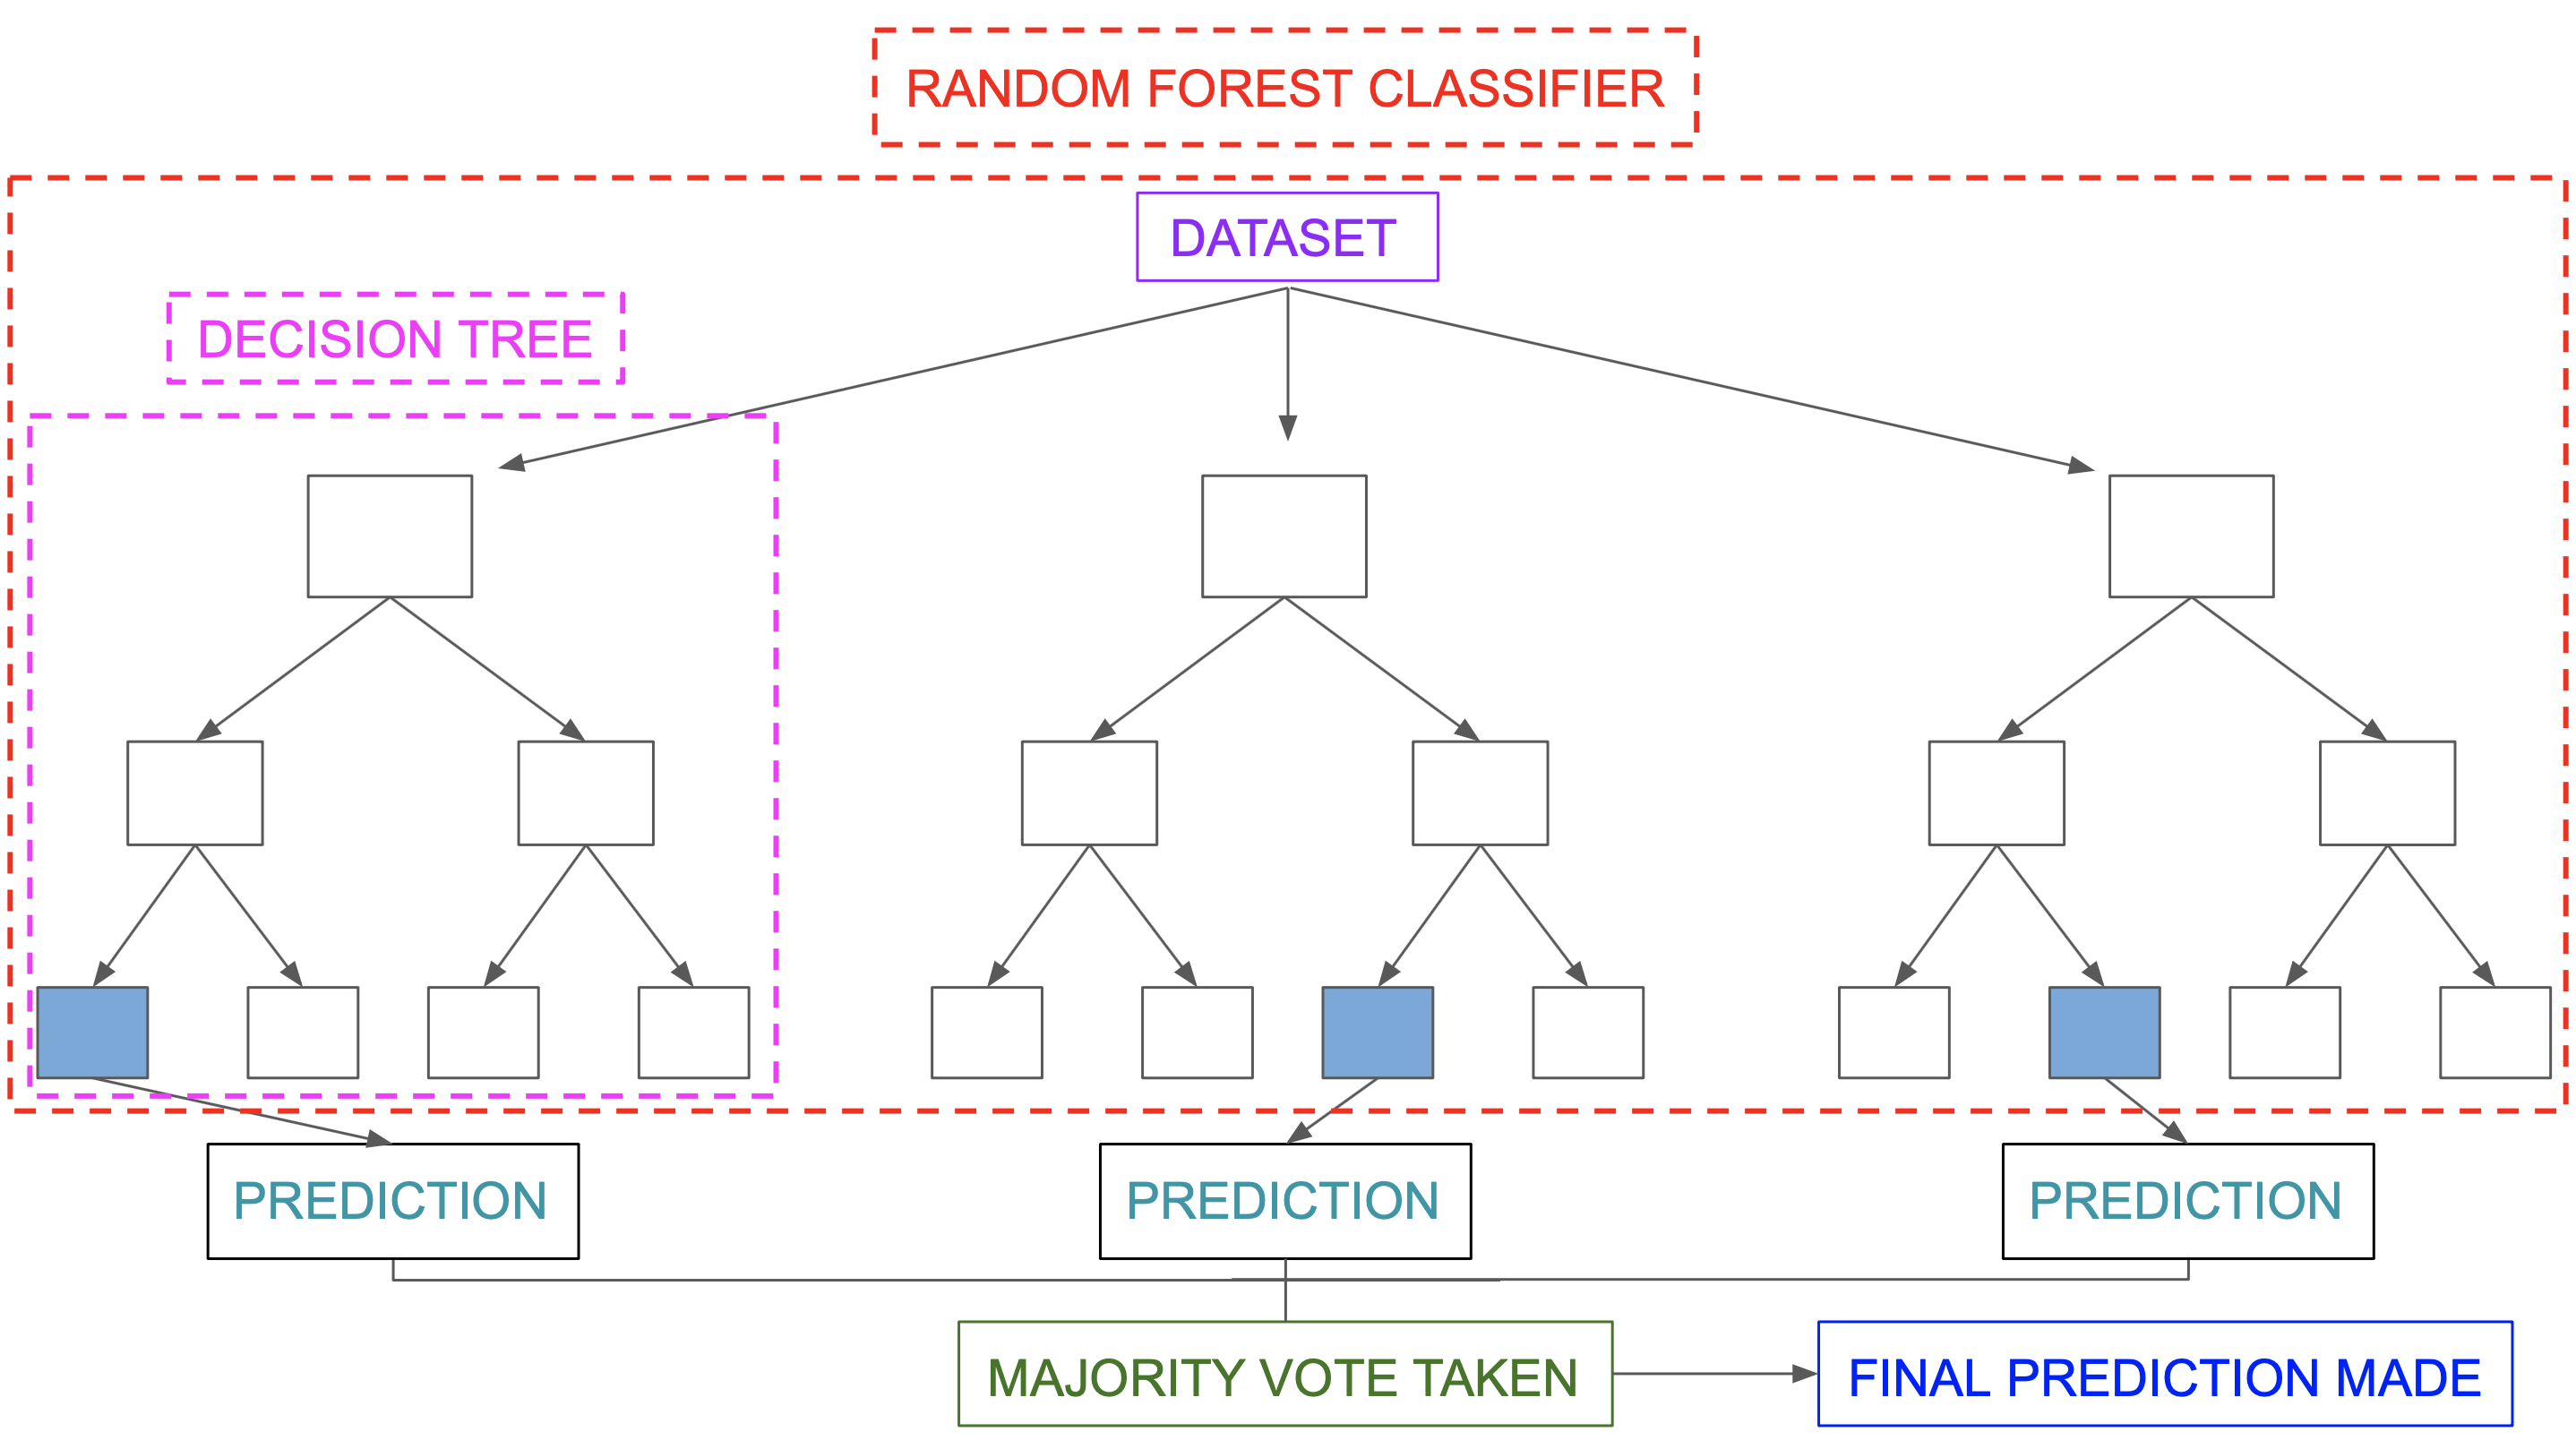
\includegraphics[width=\linewidth, height=4.8cm]{images/random-forest-classifier.png}
    \caption{Foret aléatoire}
    \label{fig:L1}
\end{figure}
\end{frame}

\subsection{Fonctionnement du K-NN}
\begin{frame}{Fonctionnement du K-NN}
\begin{figure}[H]
    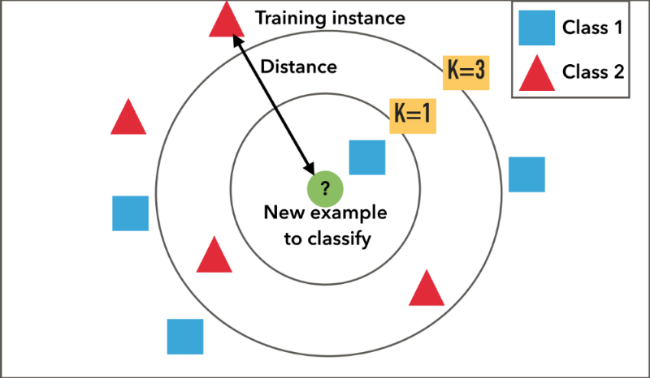
\includegraphics[width=\linewidth, height=4.8cm]{images/knn_sheama.png}
    \caption{K-Nearest Neighbor}
    \label{fig:L1}
\end{figure}
\end{frame}
\begin{frame}{Les types de distances}
\begin{itemize}
		\item Distance euclidienne
		$$d(A,X) = \sqrt{\sum_{i=1}^{n} (a_{i}-x_{i})^{2}}$$
		\item Distance de Manhattan\\
		$$d(A,X) = \sum_{i=1}^{n} \mid{a_{i}-x_{i}}\mid$$
		\item Distance de Minkowski
		$$d(A,X) = \sqrt[p]{\sum_{i=1}^{n} \mid{a_{i}-x_{i}}\mid^{p}}$$
\end{itemize}
\end{frame}
\begin{frame}{Choix du paramètre K}
\begin{itemize}
		\item Utilisation de K
		$$K=\sqrt{nombre-de-donnees }$$
		\item Choisir K suivant celui qui donne une meilleure prédiction
\end{itemize}
\end{frame}

\section{Système réalisé}
\begin{frame}{Informations données}
\begin{figure}[H]
    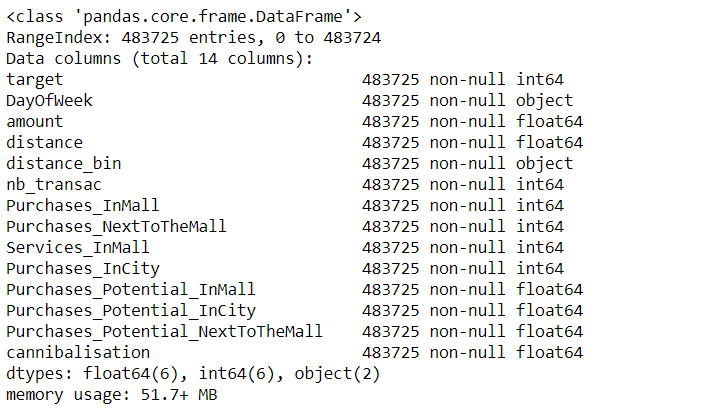
\includegraphics[width=11cm,height=4.8cm]{images/data_infos.png}
    \caption{ Les types de features}
    \label{fig:L1}
\end{figure}
\end{frame} 

%\section{Résultats obtenus}

\section{Conclusion}
  \begin{frame}
  \begin{block}{}
  Ici une conclusion qui met en valeur votre travail et indique ce qui reste à faire
  \end{block}
  \end{frame}

% éléments hors section
\begin{frame}
\frametitle{Références}
\begin{thebibliography}{9}
\bibitem{texbook}
Yingjie Tian, Yong Shi, Xiaohui Liu. RECENT ADVANCES ON SUPPORT VECTOR MACHINES RESEARCH.  in TECHNOLOGICAL AND ECONOMIC DEVELOPMENT OF ECONOM, 2012  Volume 18(1): 5–33


\bibitem{lamport94}
Jehad Ali, Rehanullah Khan, Nasir Ahmad, Imran Maqsood. Random Forest and Decision Tree. In  IJCSI International Journal of Computer Science Issues, Vol. 9, Issue 5, No 3, September 2012 ISSN (Online): 1694-0814



\end{thebibliography}
\end{frame}
\begin{frame}
\frametitle{Références}
\begin{thebibliography}{9}
\bibitem{texbook}
Gongde Guo, Hui Wang, David Bell, Yaxin Bi, and Kieran Greer. KNN Model-Based Approach in Classification. In School of Computing and Mathematics, University of Ulster Newtownabbey, BT37 0QB, Northern Ireland, UK


\bibitem{lamport94}
Ramraj S, Nishant Uzir, Sunil R  and Shatadeep Banerjee. Experimenting XGBoost Algorithm for Prediction and Classification of Different Datasets. In International Journal of Control Theory and Applications ISSN : 0974–5572 International Science Press Volume 9  •  Number 40  , 2016


\end{thebibliography}
\end{frame}
\begin{frame}
\frametitle{Références}
\begin{thebibliography}{9}
\bibitem{lamport94}
C. Mitchell Dayton. LOGISTIC REGRESSION ANALYSIS. Department of Measurement, Statistics and Evaluation.  In Room 1230D Benjamin Building University of Maryland September 1992

\end{thebibliography}
\end{frame}

\begin{frame}
  \begin{block}{}
  \centering
  Merci pour votre attention
  \end{block}
\end{frame}


\end{document}
